\section*{\hfill{}УСЛОВИЕ\hfill{}}
В пекарню приходят клиенты каждые $4\pm1$ минуты. Обслуживание на кассе просиходит $3\pm2$ минуты. Если в очередь на кассу содержит больше 5 человек, то клиент уходит. С вероятностью 10\% клиента не заинтересует ассортимент и он уйдет; 30\%~--- клиент закажет уже готовую продукцию, что приведёт к выдаче; 5\%~--- продукцию, которую по тем или иным причинам приготовить не представляется возможным, что приведёт к уходу клиента; 35\%~--- клиент закажет продукцию, которую будет необходимо и возможно приготовить. Заказ клиента с 60\% вероятностью будет маленьким, а с вероятностью 40\%~--- большим. Повар 1 и повар 2 занимаются только маленькими заказами, а повар 3~--- только большими. Время приготовления продукции каждым поваром составляет $10\pm2$ минут, $11\pm2$ минут и $20\pm4$ минут соотвественно. Выбор между поваром 1 и поваром 2 происходит по равномерному распределению. Результат приготовления попадает на выдачу. С вероятностью 5\% продукция на выдаче не понравится клиенту и он уйдёт.

Промоделировать процесс обслуживания 500 клиентов, определить вероятность отказа.

\section*{\hspace{1.25cm}1\quad{}Теоретическая часть}
На рисунке\ref{img:concept} изображена структурная схема рассматриваемой концептуальной модели.
\begin{figure}[H]
    \centering
    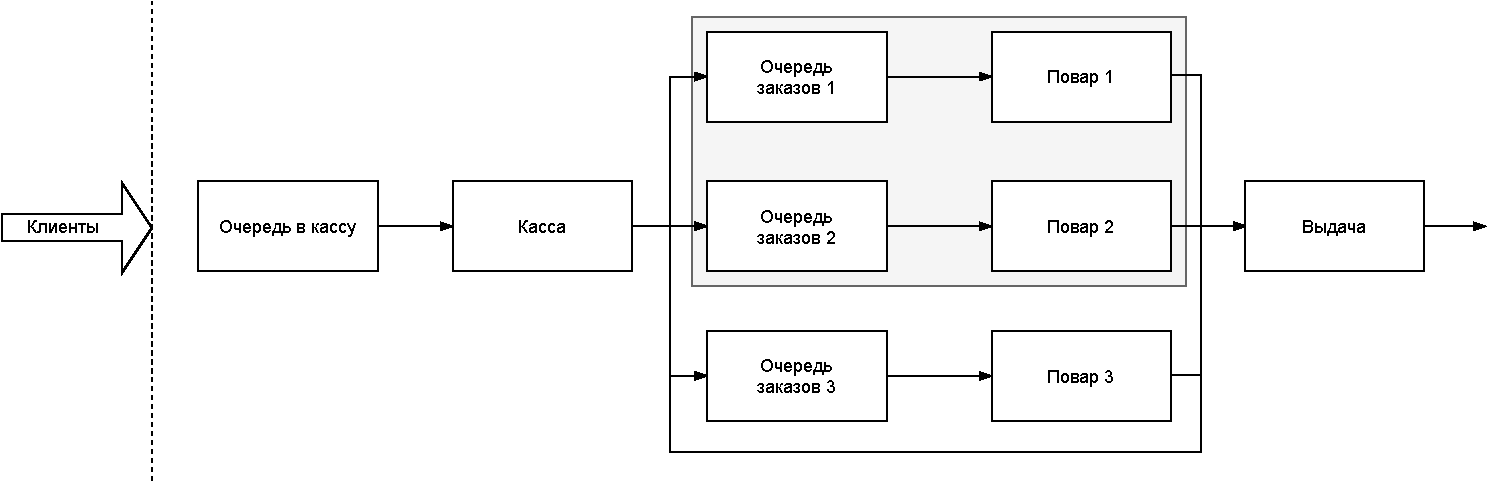
\includegraphics[width=1\textwidth]{pdf/concept.pdf}
    \caption{Структурная схема}
    \label{img:concept}
\end{figure}

\section*{\hspace{1.25cm}2\quad{}Результаты}
Вероятность отказа~--- это промежуток, поэтому прогоним модель 100 раз и выберем минимальное и максимальное значения.

На рисунке~\ref{img:results} представлены результаты выполнения программы.
\begin{figure}[H]
    \centering
    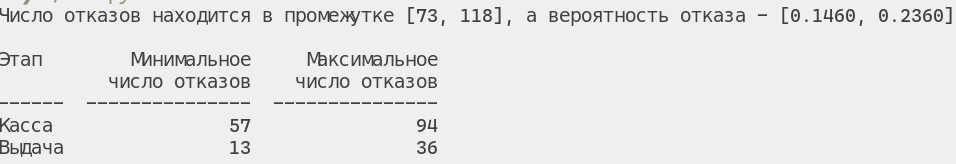
\includegraphics[width=0.6\textwidth]{images/scr01.png}
    \caption{Результаты}
    \label{img:results}
\end{figure}

\section*{\hfill{}ВЫВОД\hfill{}}
В настоящей лабораторной работе была промоделирована информационная система, в которую поступают клиенты. Эта система состоит нескольких блоков, а именно: очередь в кассу, касса, три очереди к поварам и три повара, а так же пункт выдачи. Выходными данными являются вероятность отказа и количество клиентов, отказ получивших.
